\documentclass[border=5pt]{standalone}
\usepackage{tikz}
\usetikzlibrary{calc,intersections,through}
\begin{document}
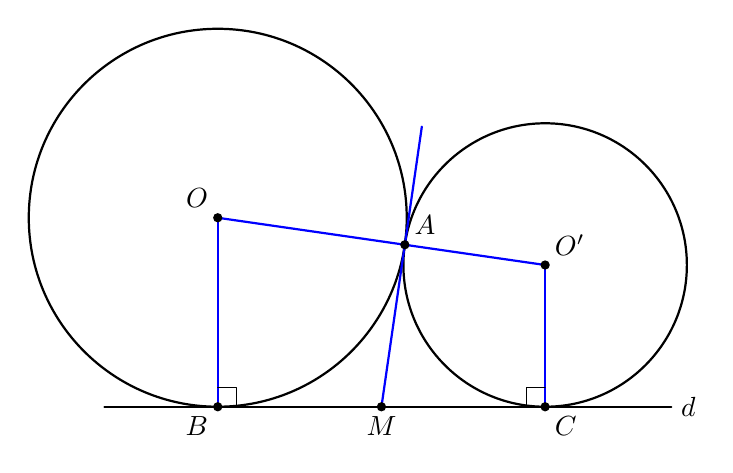
\begin{tikzpicture}[scale=1.2, line cap=round, line join=round]
  % --- Toạ độ (đã tính bằng Python) ---
  % (O) bán kính R=2, (O') bán kính R'=1.5, tiếp xúc ngoài
  % d là trục hoành (y=0)
  \coordinate (O) at (0, 2);
  \coordinate (Op) at (3.4641, 1.5);
  \coordinate (B) at (0, 0);
  \coordinate (C) at (3.4641, 0);
  \coordinate (A) at (1.9795, 1.7143);
  \coordinate (M) at (1.7321, 0);

  % --- Đường thẳng d (tiếp tuyến chung ngoài) ---
  \draw[thick] (-1.2, 0) -- (4.8, 0);

  % --- Hai đường tròn ---
  \draw[thick] (O) circle (2);
  \draw[thick] (Op) circle (1.5);

  % --- Tiếp tuyến tại A (đường MA kéo dài) ---
  % Phương tiếp tuyến tại A vuông góc OO': direction (-uy, ux)
  % ux = 3.4641/3.5 = 0.9898, uy = -0.5/3.5 = -0.1429
  % direction tiếp tuyến = (0.1429, 0.9898)
  % Kéo từ M qua A lên trên
  \draw[blue, thick] (M) -- ($(A)+(0.18, 1.25)$);

  % --- Đoạn OB vuông góc d, O'C vuông góc d (nét phụ) ---
  \draw[blue, thick] (O) -- (B);
  \draw[blue, thick] (Op) -- (C);

  % --- Đoạn OO' ---
  \draw[blue, thick] (O) -- (Op);

  % --- Ký hiệu góc vuông tại B ---
  \draw ($(B)+(0, 0.20)$) -- ($(B)+(0.20, 0.20)$) -- ($(B)+(0.20, 0)$);

  % --- Ký hiệu góc vuông tại C ---
  \draw ($(C)+(0, 0.20)$) -- ($(C)+(-0.20, 0.20)$) -- ($(C)+(-0.20, 0)$);

  % --- Chấm điểm ---
  \foreach \p in {O,Op,A,B,C,M} \fill (\p) circle (1.4pt);

  % --- Nhãn ---
  \node[above left] at (O) {$O$};
  \node[above right] at (Op) {$O'$};
  \node[above right] at (A) {$A$};
  \node[below left] at (B) {$B$};
  \node[below right] at (C) {$C$};
  \node[below] at (M) {$M$};
  \node[right] at (4.8, 0) {$d$};
\end{tikzpicture}
\end{document}
